\documentclass[a4paper, 12pt]{report}

\usepackage[spanish]{babel}
\usepackage[utf8]{inputenc}
\usepackage[left=4cm, right=4cm, top=4cm]{geometry}
\usepackage{textcomp}
\usepackage{booktabs}
\usepackage{amssymb}
\usepackage{bussproofs}
\usepackage{fancyhdr}
\usepackage{graphicx}
\usepackage{amsmath}

\usepackage{hyperref}
\hypersetup{
    colorlinks=true,
    linkcolor=blue,
    filecolor=magenta,
    urlcolor=cyan,
}

\pagestyle{fancy}
\lhead{Almeida, Figueroa \& Ibarra}
\chead{Tarea 2}
\rhead{\today}

\begin{document}
\begin{titlepage}
    \centering
    {\scshape\Huge Universidad Nacional Autónoma de México \par}
    \vspace{1.25cm}
    {\scshape\huge Fundamentos de Bases de Datos\par}
    \vspace{1.25cm}
    {\huge\bfseries Tarea 2: Modelo Entidad-Relación\par}
    \vspace{1.25cm}
    {\Large\textsc Almeida Rodríguez Jerónimo\par}
    \vspace{.1cm}
    {\large\texttt{418003815}\par}
    \vspace{0.25cm}
    {\Large\textsc Figueroa Sandoval Gerardo Emiliano\par}
    \vspace{.1cm}
    {\large\texttt{315241774}\par}
    \vspace{0.25cm}
    {\Large\textsc Ibarra Moreno Gisselle \par}
    \vspace{.1cm}
    {\large\texttt{315602193}\par}
    \vspace{1.5cm}
    \vfill
    \begin{figure}[hb!]
        
\includegraphics[width=.3\textwidth]
            {../logos/escudo_f-ciencias.png}\hfill
        
\includegraphics[width=.3\textwidth]
            {../logos/Escudo_UNAM.png}\hfill
    \end{figure}
\end{titlepage}
\begin{enumerate}
\item[1)]{
\begin{enumerate}
    \item[i)]{Un conjunto de entidades débiles siempre se puede convertir en un
        conjunto de entidades fuertes añadiéndole a sus atributos la llave
        primaria del conjunto de entidades fuertes a las que está asociado.
        Describe qué tipo de redundancia resultaría si se realizara dicha
        conversión.\\
        La redundancia que resultaría sería que cualquier dato que se haya
        tomado cómo llave primaria en la entidad principal estaría repetida
        tantas veces cómo entidades débiles asociadas a dicha entidad.
    }
    \item[ii)]{}
    \item[iii)]{Explica el concepto de agregación en el modelo E/R y
        proporciona un par de ejemplos.\\

         Es un concepto de abstracción, permite construir entidades
         de más alto nivel compuestas a partir de otras más pequeñas.\\
        \textbf{Ejemplo1:}\\
        Un científico puede trabajar en varios proyectos y un proyecto
        tiene como participante a varios científicos. Además un
        científico pública un artículo sobre el proyecto en el que
        trabajo.\\
        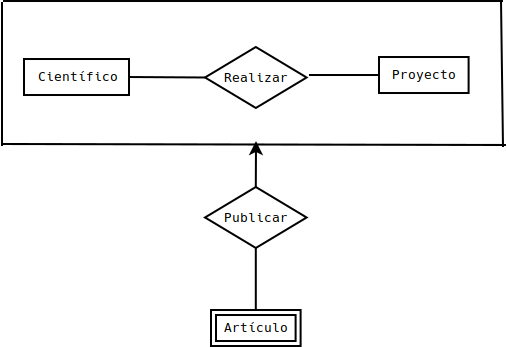
\includegraphics[scale= 0.5]{Ejemplo1.png}\\
        \textbf{Ejemplo2:}\\
        Un empleado trabaja en un departamento en una sucursal, la
        sucursal, los departamentos y el empleado es dirigido por un
        director.\\
        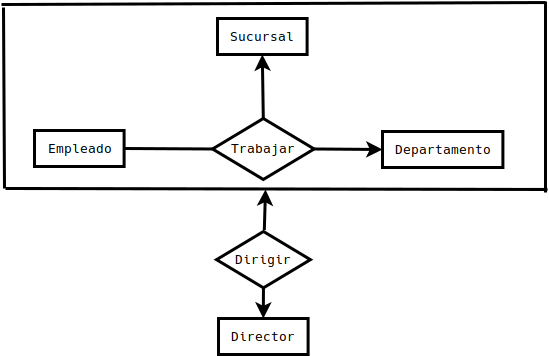
\includegraphics[scale= 0.5]{Ejemplo2.png}}
    \item[iv)]{}
\end{enumerate}
}
\item[2)]{
\begin{enumerate}
    \item[a)]{}
    \item[b)]{
        \begin{figure}[hb!]
            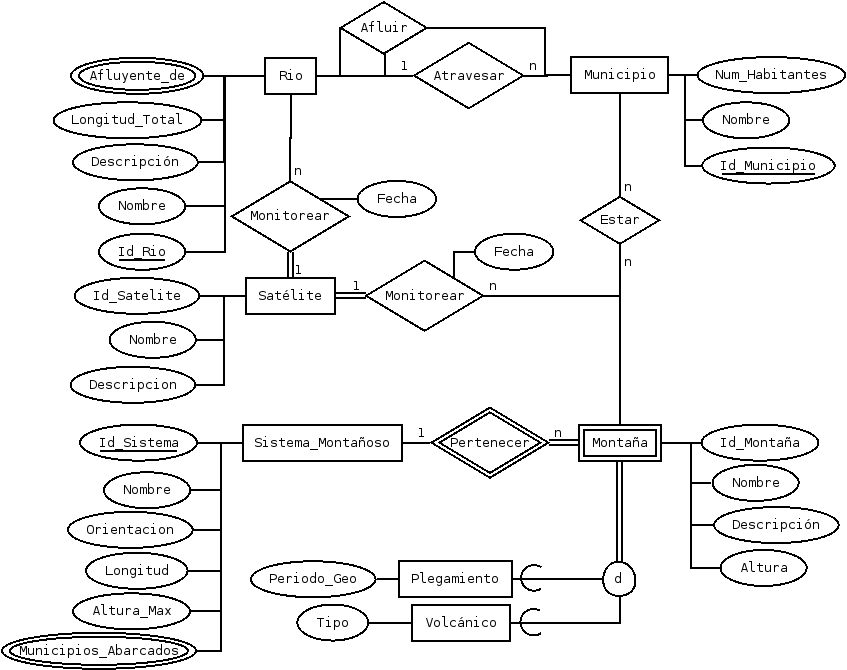
\includegraphics[width=\textwidth]
                {SIG.png}\hfill
            \caption{Base de Datos SIG}
        \end{figure}
    }
    \item[c)]{\textbf{Ingeniería inversa}:
        Una compañía celular requiere una base de datos para realizar
        un seguimiento de sus clientes, sus planes de suscripción y
        los teléfonos móviles que  están  utilizando.  El diagrama
        E/R de  la  siguiente figura  muestra  entidades  de  interés
        para  la  compañía  y  las  relaciones  entre  ellas.
        Tomando  como base el esquema proporcionado, responde a las
        siguientes preguntas justificando tu respuesta. Para cada
        pregunta, identificar el o los elementos en el diagrama E/R
        que utilizaste para tu respuesta. En caso de que alguna
        pregunta no se cumpla en el diagrama actual, indica las
        modificaciones que deberían hacerse para que se permita dicho
        comportamiento.\\
        \begin{enumerate}
            \item ¿Un cliente puede tener un número ilimitado de planes?\\
            Sí, ya que la relación de poseer es de muchos a muchos, por
            lo que un cliente puede tener más de un plan.
            \item ¿Un cliente puede existir sin un plan?\\
            Sí, ya que la relación de poseer, no es total del lado del
            cliente, por lo que no es necesario que tenga un plan.
            \item ¿Es posible crear un plan sin saber quién es el
            cliente?\\
            No, la relación que va desde el plan hasta poseer es total,
            es decir un plan siempre tiene un cliente, por lo que es
            necesario que se sepa quién es el cliente al que va
            dirigido.
            \item ¿El operador quiere limitar los tipos de dispositivos
            que se pueden vinicular a un tipo de plan específico?\\
            Sí, ya que un teléfono incluye solo un plan.
            \item ¿Es posible mantener los datos relativos a un
            teléfono, sin conectarlo a un plan?\\
            Sí, ya que la participación de un teléfono a incluir no es
            total, por lo que el teléfono no necesita tener un plan.
            \item ¿Puede un teléfono asociar varios planes?\\
            No, no puede, ya que la relación incluir es uno a muchos,
            es decir un plan puede incluir varios teléfonos pero un
            teléfono solo puede tener un plan.
            \item Supongamos que existe un tipo de teléfono que puede
            utilizar múltiples sistemas operativos. ¿Este tipo de
            situación podría tener cabida dentro del modelo incluido
            en la figura?\\
            Sí, solo se necesitaría cambiar la relación de tener que va
            desde tipo de teléfono a sistema operativo a una relación
            muchos a muchos
            \item ¿La empresa capaz de realizar un seguimiento de un
            fabricante sin mantener información sobre sus teléfonos?\\
            No, no puede, ya que desde el cliente o desde el plan,
            no se puede identificar al fabricante ya que no están
            relacionados, para identificar el fabricante, se necesitan
            los datos del teléfono.
            \item ¿Puede el mismo sistema operativo utilizarse en
            múltiples tipos de dispositivos?\\
            Sí, ya que la relación tener entre tipo de teléfono y
            sistema operativo es muchos a uno, es decir, un sistema
            operativo puede estar en varios tipos de teléfonos, pero
            un tipo de teléfono sólo tiene un sistema operativo.
            \item Hay dos relaciones entre el Cliente y el Plan. Explicar en qué
                difieren.\\
            Poseer es una relación con cardinalidad muchos a muchos,
            además tiene participación parcial de parte del cliente y
            total de parte del plan.\\
            Administrar es una relación de uno a muchos con
            participación total de los dos lados.
            \item Caracterizar el grado y la cardinalidad de la
            relación que une al cliente a sí mismo. Explicar su
            significado.\\
            Tiene cardinalidad uno a muchos con participación total de
            un lado y parcial del otro, es decir un cliente tiene muchos
            clientes pero un cliente solo tiene un cliente,
            además un cliente siempre tiene un cliente y a la vez un
            cliente puede no tener un cliente.
            \item ¿Es posible vincular un teléfono a un cliente
            específico en un plan con múltiples clientes?\\
            Sí, ya que un plan es administrado solo por un cliente.
            \item ¿Puede la compañía rastrear un teléfono sin identificar su
            sistema operativo?\\
            Sí ya que no depende del sistema operativo, hay otras
            formas de identificar un teléfono.

        \end{enumerate}
    }
\end{enumerate}
}
\end{enumerate}


\begin{thebibliography}{20}
\end{thebibliography}

\end{document}
